\documentclass[11pt]{article}
\usepackage[utf8]{inputenc}
\usepackage[T1]{fontenc}
\usepackage[margin=1in]{geometry}
\usepackage{amsmath,amssymb,amsthm}
\usepackage{booktabs}
\usepackage{array}
\usepackage{url}
\usepackage{microtype}
\usepackage{graphicx}
\usepackage{caption}
\usepackage{xcolor}
\usepackage{listings}
\usepackage[hidelinks]{hyperref}
\makeatletter\g@addto@macro{\UrlBreaks}{\do\_\do\.\do\/}\makeatother
\emergencystretch=3em
\tolerance=2000
% generated by gen_inputs.py; do not edit
\newcommand{\KTVdlmfErr}{1.8\times10^{-16}}
\newcommand{\KTVmixErr}{2.4\times10^{-15}}
\newcommand{\KTVnpts}{28}
\newcommand{\KTKernelErr}{1.8\times10^{-15}}
\newcommand{\KTBoxDiff}{6.9\times10^{-14}}
\newcommand{\KTLitTri}{5.0\times10^{-10}}
\newcommand{\KTLitSq}{8.3\times10^{-10}}
\newcommand{\KTdEnine}{3.14\times10^{-9}}
\newcommand{\KTSlopeEight}{0.99999998}
\newcommand{\KTSlopeTwo}{0.98585}
\newcommand{\KTAlphaSpread}{3.5\times10^{-15}}
\newcommand{\KTNegSign}{5.3\times10^{-2}}
\newcommand{\KTNegBg}{0.216}
\newcommand{\KTWrongKernelE}{+1.9605}
\newcommand{\KTScalingErr}{9.7\times10^{-16}}
\newcommand{\KTLogGas}{0.0052922513}
\newcommand{\KTLogGasDevTwo}{-3.4\times10^{-3}}
\newcommand{\KTLogGasDevSix}{-3.4\times10^{-7}}
\newcommand{\KTMinGap}{5.27\times10^{-5}}
\newcommand{\KTNScan}{51}
\newcommand{\KTAllGapsPos}{yes}
\newcommand{\KTEtriC}{-1.9605157893}
\newcommand{\KTEsqC}{-1.9501324600}
\newcommand{\KTGapC}{1.0383\times10^{-2}}
\newcommand{\KTTestsPassed}{28}
\newcommand{\KTTestsFailed}{0}
\newcommand{\KTTestsIgnored}{1}
\newcommand{\KTScanSame}{bit-identical}
\newcommand{\KTRecompileStatus}{rc 0 in 848.1 s, axiom output identical to the producer's}
\newcommand{\KTShaKeldysh}{1bac0d410d366614c8d287f7ea95d495aa0ee09c4782cfa0d5b691a3048647f2}
\newcommand{\KTShaControls}{d7e5516fe00a6599a181d5a394dde70a66c533d0a2693b78b9035281801f0606}
\newcommand{\KTShaYukawa}{a16397de179837dd2119cf09c1b3086db7650b9b8bbaeb322f2d531936c033cf}
\newcommand{\KTRouteEPosErr}{2.1\times10^{-17}}
\newcommand{\KTRouteENegInner}{0.37}
\newcommand{\KTRouteENegSub}{0.82}
\newcommand{\KTMoSElevenTri}{-73.77}
\newcommand{\KTMoSElevenGap}{0.431}

\lstset{basicstyle=\ttfamily\footnotesize,columns=fullflexible,keepspaces=true,breaklines=true,
  frame=single,framesep=3pt,xleftmargin=4pt,xrightmargin=4pt,upquote=true,
  keywordstyle=\bfseries,morekeywords={theorem,lemma,def,noncomputable,structure,where,fun,Prop,axiom},
  escapeinside={(*@}{@*)}}
\newtheorem{theorem}{Theorem}
\newtheorem{lemma}[theorem]{Lemma}
\theoremstyle{remark}
\newtheorem{remark}[theorem]{Remark}
\newcommand{\R}{\mathbb{R}}
\newcommand{\tier}[1]{\textsf{[#1]}}
\newcommand{\erfcx}{\operatorname{erfcx}}
\newcommand{\lean}[1]{\texttt{#1}}
\makeatletter\newcommand{\tabinput}[1]{\@@input #1 }\makeatother

\title{The Rytova--Keldysh interaction is a positive Gaussian mixture:\\ kernel-checked admissibility for planar
universal optimality\\ and Keldysh-jellium Madelung energies of TMD Wigner lattices}
\author{Xavier Callens (SocrateAI Lab)}
\date{Preprint v1, 2026-10-25}
\hypersetup{pdftitle={The Rytova-Keldysh interaction is a positive Gaussian mixture: kernel-checked admissibility for
planar universal optimality and Keldysh-jellium Madelung energies of TMD Wigner lattices}, pdfauthor={Xavier Callens}}

\begin{document}
\maketitle

\noindent\textbf{AI-assistance disclosure.} This preprint, its Lean code, its Rust and Python code and its ledger were
produced by AI agents (Claude, Anthropic) under the author's direction. The author is responsible for the content. No
human has yet audited the Lean statements for adequacy, and no human referee has checked the hand proofs.

\begin{abstract}
In units $e^2/(4\pi\varepsilon_0)=1$, the Rytova--Keldysh potential of a freestanding two-dimensional semiconductor is
$V(r)=\frac{\pi}{2r_0}[\mathbf H_0-Y_0](r/r_0)$. We give a human proof (\tier{C}, not machine-checked) that, as a
function of $t=r^2$, it is a positive mixture of Gaussians with weight
$w(a)=r_0^{-1}e^{a/r_0^2}\operatorname{erfc}(\sqrt a/r_0)$. It is therefore completely monotone
in $t$, which is the class covered by the openai/math theorem on universal optimality of the triangular
lattice~\cite{oai}.

\textbf{Tier A (kernel-checked in Lean~4.34.1).} The axiom footprint is $\{$\lean{propext}, \lean{Classical.choice},
\lean{Quot.sound}$\}$ and planted controls are caught. We prove a generic lemma: every positive exponential mixture with
finite moments satisfies upstream's \lean{AdmissiblePotential}. For the mixture-\emph{defined} Keldysh potential we
prove admissibility, strict positivity, and a Gaussian-regularised variant. Applying upstream's
\lean{universal\_energy\_minimum} then gives the triangular-lattice inequalities. Every triangular-lattice statement
is conditional on that upstream theorem, which is AI-generated and not peer reviewed, and on the fidelity of its
definitions. The unregularised inequality is expected to read $\top\le\top$ \tier{C}. Finiteness of the regularised
energy is not proved \tier{C}.

\textbf{Tier C.} That the mixture equals the Struve form is a human proof, given here step by step.

\textbf{Tier X.} Floating-point checks only. A new rusty-SUNDIALS module computes Keldysh-jellium Madelung energies of
the triangular and square Wigner lattices by an Ewald split in the mixture variable. It reproduces the Coulomb values
at $r_0=0$ and the Dedekind-$\eta$ log-gas gap as $r_0\to\infty$. It finds $E_\mathrm{sq}-E_\mathrm{tri}>0$ at all
\KTNScan{} sampled $r_0\sqrt n$. For MoS$_2$, MoSe$_2$, WS$_2$ and WSe$_2$ in vacuum we take $r_0$ from published
polarizabilities \tier{L}. A HuggingFace C2DB-derived dataset is used to identify the 2H phases and to cross-check
lattice constants. It contains no polarizabilities.

None of this is a breakthrough. Complete monotonicity of $V$ follows quickly from textbook integrals. What is new is
the machine-checked admissibility against upstream's definition, and the tiered bookkeeping.
\end{abstract}

\paragraph{Tiers.} \tier{A}: kernel-checked Lean, with axioms within the allowlist and planted controls caught.
\tier{L}: a cited source, quoted in the ledger (prose as extracted, mathematics transcribed linearly, elisions
marked). This is looser than the strict Elenchus \texttt{citation\_check}, which accepts only theorem-kind statements
quoted verbatim: KT-L-0001, KT-L-0002 and KT-L-0005 (an equation, table values and a README) and the Remark~1.5 numbers
in KT-L-0003 would be refused on kind, and the linearised mathematics would not match verbatim. Sandier--Serfaty
Theorem~2 passes that strict check (Stage-4 audit). \tier{C}: an argument or human proof that is not
machine-checked. \tier{X}: floating-point exploration, which never supports a claim. Ledger identifiers
(\texttt{KT-A-0006} and so on) refer to \texttt{ledger/ledger.json} (Section~\ref{sec:ledger}). A Tier~A tag attaches to
the Lean statement, never to its physical gloss.

\section{Setting}\label{sec:setting}
Berkelbach, Hybertsen and Reichman~\cite{bhr} write the in-plane interaction of charges in a monolayer transition-metal
dichalcogenide (TMD) between dielectrics $\varepsilon_1,\varepsilon_2$ as
$V_{2D}(\rho)=\frac{\pi e^2}{(\varepsilon_1+\varepsilon_2)\rho_0}[\mathbf H_0(\rho/\rho_0)-Y_0(\rho/\rho_0)]$. They
call it ``a form derived by Keldysh''~\cite{keldysh}. In vacuum the screening length is $\rho_0=2\pi\chi_{2D}$, after
Cudazzo et al.~\cite{cudazzo} \tier{L, KT-L-0001}. With $\varepsilon_1=\varepsilon_2=1$ and $e^2/(4\pi\varepsilon_0)=1$
this is
\begin{equation}\label{eq:V}
V(r)=\frac{\pi}{2r_0}\,\mathbf K_0(r/r_0),\qquad \mathbf K_0=\mathbf H_0-Y_0\ \text{(DLMF 11.2.5~\cite{dlmf})},\qquad
\widehat V(k)=\frac{2\pi}{k(1+r_0k)}
\end{equation}
\tier{C, KT-C-0004}. The Fourier transform uses $\widehat V(k)=\int_{\R^2}V(|x|)e^{-ik\cdot x}\,d^2x$, and the limit
$r_0\to0$ recovers the Coulomb kernel $2\pi/k$.

Upstream~\cite{oai} calls $g:\R\to\R$ \emph{admissible} if it is $C^\infty$ on $(0,\infty)$, $g\ge0$ there, and
$(-1)^n g^{(n)}\ge0$ for all $n$. The pair interaction is $g(|x-y|^2)$, so $g$ is a function of the \emph{squared}
distance. Upstream proves that the triangular lattice $A$ of density one has the least lower energy among locally
finite density-one configurations. Energies are taken in $[0,\infty]$ (Listing~\ref{lst:up}) \tier{A, KT-A-0001}.

\lstinputlisting[caption={Upstream definition and theorem (openai/math, pinned copy; proof elided).},label=lst:up]{gen/upstream.lst}
\texttt{gen\_inputs.py} extracts the listings from the pinned sources into \texttt{gen/*.lean}, byte for byte. The
typeset \texttt{gen/*.lst} copies differ only in that each non-ASCII symbol is escaped to its LaTeX glyph.

\section{Step-by-step human demonstration}\label{sec:human}
This section is written for a strong undergraduate. Each step gives the mathematical statement and its proof, then the
Lean declaration that checks it. Steps 0--6 are mirrored in Lean \tier{A}. Step~7, the link to the Struve function, is
not formalized; it is \tier{C}.

\paragraph{Step 0: the weight.} For $x\ge0$ put
$\erfcx(x)=\frac{2}{\sqrt\pi}\int_0^\infty e^{-(y^2+2xy)}\,dy$. Substituting $s=y+x$ gives
$\erfcx(x)=e^{x^2}\frac{2}{\sqrt\pi}\int_x^\infty e^{-s^2}ds=e^{x^2}\operatorname{erfc}(x)$, the usual scaled
complementary error function. Lean \emph{defines} \lean{erfcx} by the integral, because Mathlib at this pin has no
$\operatorname{erfc}$. The two forms agree numerically: the max relative error is $1.34\times10^{-31}$ at seven points,
and a perturbed integrand ($2xy\to xy$) is off by at least $5.6\times10^{-3}$ at the six points with $x>0$; at $x=0$
the perturbation has no effect \tier{X, KT-X-0001}. For $r_0>0$ set
$w(a)=r_0^{-1}\erfcx(\sqrt a/r_0)$.

\begin{lemma}[bounds on the weight]\label{lem:w}
For $x\ge0$, $0<\erfcx(x)\le1$. For $x>0$, $\erfcx(x)\le 1/(\sqrt\pi\,x)$. Hence, for $a>0$,
$0<w(a)\le 1/r_0$ and $w(a)\le 1/(\sqrt\pi\sqrt a)$.
\end{lemma}
\begin{proof}
The integrand is positive and continuous, so $\erfcx(x)>0$. For $y>0$ and $x\ge0$ we have $y^2+2xy\ge y^2$, so the
integral is at most $\int_0^\infty e^{-y^2}dy=\sqrt\pi/2$, which gives $\erfcx\le1$. If $x>0$, drop $y^2$ instead:
$\int_0^\infty e^{-2xy}dy=1/(2x)$, so $\erfcx(x)\le\frac{2}{\sqrt\pi}\cdot\frac1{2x}$. For $w$, substitute
$x=\sqrt a/r_0$: $w\le r_0^{-1}\cdot r_0/(\sqrt\pi\sqrt a)$.
\end{proof}
\noindent Lean: \lean{erfcx\_le\_one}, \lean{erfcx\_le\_inv}, \lean{erfcx\_pos}, \lean{w\_le}, \lean{w\_le\_sqrt}
\tier{A, KT-A-0005}.

\paragraph{Step 1: every moment is finite.}
\begin{lemma}\label{lem:mom}
For $r_0>0$, $n\in\mathbb N$ and $c>0$, the function
$F_n(a)=(4a)^{-n}e^{-c/(4a)}\,w(a)/(2a)$ is integrable on $(0,\infty)$.
\end{lemma}
\begin{proof}
Split at $a=1$. \emph{On $(0,1]$:} put $u=1/(4a)$, so that $w(a)/(2a)=2u\,w(a)$ and
$F_n=2w(a)\,u^{n+1}e^{-cu}$. From $e^{cu}\ge (cu)^N/N!$ we get $u^Ne^{-cu}\le N!/c^N$. So
$F_n\le 2r_0^{-1}(n+1)!/c^{n+1}$, a constant, and a bounded measurable function on an interval of finite length is
integrable. \emph{On $(1,\infty)$:} here $u\le 1/4\le1$, so $u^n\le1$ and $e^{-cu}\le1$. Then
$F_n\le w(a)/(2a)\le \frac{1}{2\sqrt\pi}a^{-3/2}$ by Lemma~\ref{lem:w}, and $\int_1^\infty a^{-3/2}da=2<\infty$.
\end{proof}
\noindent Lean: \lean{pow\_mul\_exp\_neg\_le} (the bound $u^Ne^{-cu}\le N!/c^N$) and \lean{keldysh\_integrable}, which
uses exactly the split $(0,1]\cup(1,\infty)$ \tier{A, KT-A-0005}.

\paragraph{Step 2: the generic lemma.} Let $(\alpha,\mu)$ be a measure space. Let $k,m$ be measurable with $k\ge0$,
$m\ge0$ $\mu$-a.e., and suppose $\int k^ne^{-ck}m\,d\mu<\infty$ for all $n$ and all $c>0$. Put
$G_n(t)=\int(-k)^ne^{-tk}m\,d\mu$ and $g=G_0$.
\begin{theorem}\label{thm:generic}
$g$ is admissible, and $g^{(n)}(t)=G_n(t)$ for $t>0$.
\end{theorem}
\begin{proof}
Fix $t>0$ and let $s$ range over $(t/2,\infty)$, a neighbourhood of $t$. The $s$-derivative of
$(-k)^ne^{-sk}m$ is $(-k)^{n+1}e^{-sk}m$. Its absolute value is $k^{n+1}e^{-sk}m\le k^{n+1}e^{-(t/2)k}m$, because
$s\ge t/2$ and $k\ge0$. The right side does not depend on $s$, and it is integrable by hypothesis with $c=t/2$. So the
theorem on differentiation under the integral sign (dominated convergence) gives $G_n'(t)=G_{n+1}(t)$. Induction on
$n$ then shows $G_0\in C^N(0,\infty)$ for every $N$, and $g^{(n)}=G_n$ on $(0,\infty)$. Finally
$(-1)^nG_n(t)=\int k^ne^{-tk}m\,d\mu\ge0$, since the integrand is nonnegative a.e.; $n=0$ gives $g\ge0$.
\end{proof}
\noindent Lean: \lean{hasDerivAt\_G} (via Mathlib's \lean{hasDerivAt\_integral\_of\_dominated\_loc\_of\_deriv\_le} on
\lean{Ioi (t/2)}), \lean{contDiffOn\_G}, \lean{iteratedDeriv\_G}, \lean{G\_sign}, \lean{laplace\_admissible},
\lean{laplace\_iteratedDeriv} \tier{A, KT-A-0003}. Nonnegativity of $m$ is essential. The Lean negative control
\lean{signedMix\_not\_admissible} shows that $e^{-t}-2e^{-2t}$, a mixture with a negative weight, is not admissible,
since it is negative at $t=\log\frac32$. The positive control \lean{expNeg\_admissible} is the Dirac instance
\tier{A, KT-A-0004}.

\paragraph{Step 3: the Keldysh instance.} Take $\mu$ to be Lebesgue measure on $(0,\infty)$, $k(a)=1/(4a)$ and
$m(a)=w(a)/(2a)$. Lemma~\ref{lem:mom} is exactly the moment hypothesis, and
$e^{-tk(a)}m(a)=\frac{w(a)}{2a}e^{-t/(4a)}$. So Theorem~\ref{thm:generic} applies to
\begin{equation}\label{eq:mix}
\mathcal K_{r_0}(t)=\int_0^\infty\frac{w(a)}{2a}\,e^{-t/(4a)}\,da ,
\end{equation}
and $(-1)^n\mathcal K^{(n)}_{r_0}(t)=\int_0^\infty (4a)^{-n}\frac{w(a)}{2a}e^{-t/(4a)}da\ge0$. Lean:
\lean{keldysh\_data}, \lean{keldysh\_admissible} \tier{A, KT-A-0006}.

\paragraph{Step 4: non-vacuity.} In Lean the Bochner integral of a non-integrable function is $0$, and $0$ is
admissible. So admissibility alone could be vacuous. But for $t>0$ the integrand in~\eqref{eq:mix} is strictly positive
on $(0,\infty)$ and integrable (Lemma~\ref{lem:mom} with $n=0$, $c=t$). A nonnegative integrable function whose support
has positive measure has positive integral, so $\mathcal K_{r_0}(t)>0$. Lean: \lean{keldysh\_pos}
\tier{A, KT-A-0006}.

\paragraph{Step 5: products.} If $f,h$ are admissible, then by Leibniz's rule
\[(-1)^n(fh)^{(n)}=\textstyle\sum_j\binom nj\,[(-1)^jf^{(j)}]\,[(-1)^{n-j}h^{(n-j)}]\ge0,\]
so $fh$ is admissible. With
$h=e^{-\varepsilon t}$ ($\varepsilon\ge0$, Step 2), the Gaussian-regularised
$\mathcal K_{r_0}(t)e^{-\varepsilon t}$ is admissible. Lean: \lean{admissible\_mul} (H2 lane, imported) and
\lean{keldyshReg\_admissible} \tier{A, KT-A-0002, KT-A-0008}.

\paragraph{Step 6: the triangular-lattice corollaries.} Upstream's theorem gives, for every locally finite density-one
$C$, $\mathrm{latticeEnergy}(\mathcal K_{r_0})\le\mathrm{energy}(\mathcal K_{r_0},C)$ and the same for the regularised
interaction. These are \lean{triangular\_keldysh\_optimal} and \lean{triangular\_keldyshReg\_optimal}
\tier{A, KT-A-0007, KT-A-0008}, conditional on upstream. They need careful reading. $V(r)\sim1/r$ at large $r$, and
$\sum_{0<|x|\le R}1/|x|$ grows like $R$ over a planar lattice. So $\mathrm{latticeEnergy}(\mathcal K_{r_0})=\top$ is
expected, and the first inequality then reads $\top\le\top$ \tier{C, KT-C-0002}. It is neither proved nor refuted in
Lean. For $\varepsilon>0$ the regularised sum should be finite \tier{C, KT-C-0003}, which would make the second
inequality informative. Lean does not prove that finiteness. The physically relevant neutralised (jellium) energy is
not covered by either statement (Section~\ref{sec:num}).

\paragraph{Step 7: the mixture is the Rytova--Keldysh potential \tier{C, KT-C-0001}.}
\begin{theorem}[not machine-checked]\label{thm:ident}
For $r_0>0$ and $r>0$, $V(r)=\mathcal K_{r_0}(r^2)$, with $V$ as in~\eqref{eq:V}.
\end{theorem}
\begin{proof}
Every integrand below is nonnegative, so all interchanges of integrals are justified by Tonelli's theorem. This route
was suggested by the Stage-4 audit (an AI agent, not a human referee).

\emph{(a) A Laplace form in $r$.} DLMF 11.5.2 with $\nu=0$ gives
$\mathbf K_0(z)=\frac2\pi\int_0^\infty e^{-zu}(1+u^2)^{-1/2}du$ for $\Re z>0$ \tier{L, KT-L-0004}. With $z=r/r_0$,
\[V(r)=\frac1{r_0}\int_0^\infty e^{-ru/r_0}\,(1+u^2)^{-1/2}\,du .\]
This alone shows that $V$ is completely monotone in $r$.

\emph{(b) Subordination.} For $\rho>0$ and $t>0$,
$e^{-\rho\sqrt t}=\int_0^\infty e^{-ta}\frac{\rho}{2\sqrt\pi}a^{-3/2}e^{-\rho^2/(4a)}\,da$. This is the Laplace
transform of the L\'evy density, a standard formula that we use without a citation. Take $\rho=u/r_0$ and $t=r^2$,
insert it into (a), and exchange the $u$ and $a$ integrals (Tonelli):
\[V(r)=\int_0^\infty e^{-ta}\,\frac{a^{-3/2}}{2\sqrt\pi\,r_0^2}\left[\int_0^\infty\frac{u}{\sqrt{1+u^2}}
e^{-\lambda u^2}du\right]da,\qquad \lambda=\frac1{4r_0^2a}.\]

\emph{(c) The inner integral is elementary.} Substitute $v=\sqrt{1+u^2}$, so that $dv=u(1+u^2)^{-1/2}du$:
\[\int_0^\infty\frac{u}{\sqrt{1+u^2}}e^{-\lambda u^2}du=e^{\lambda}\int_1^\infty e^{-\lambda v^2}dv
=\frac12\sqrt{\frac\pi\lambda}\,e^{\lambda}\operatorname{erfc}(\sqrt\lambda)=\frac12\sqrt{\frac\pi\lambda}\,
\erfcx(\sqrt\lambda).\]
With $\sqrt{\pi/\lambda}=2r_0\sqrt{\pi a}$ this gives
$V(r)=\int_0^\infty e^{-ta}\rho(a)\,da$ with $\rho(a)=\dfrac{\erfcx\!\big(1/(2r_0\sqrt a)\big)}{2r_0a}$.

\emph{(d) Change of variable.} Put $a=1/(4b)$, so $da=db/(4b^2)$ in absolute value and $e^{-ta}=e^{-t/(4b)}$. Then
$\rho(a)\,da=\frac{4b\,\erfcx(\sqrt b/r_0)}{2r_0}\cdot\frac{db}{4b^2}=\frac{w(b)}{2b}\,db$, hence
$V(r)=\int_0^\infty\frac{w(b)}{2b}e^{-r^2/(4b)}db=\mathcal K_{r_0}(r^2)$.

\emph{(e) A second route, kept as a cross-check.} One can also invert the radial Fourier transform of $\widehat V$. Here
$V\notin L^1(\R^2)$ and $\widehat V\notin L^1(\R^2)$, so the inversion
$V(r)=\frac1{2\pi}\int_0^\infty\widehat V(k)J_0(kr)k\,dk=\int_0^\infty\frac{J_0(kr)}{1+r_0k}dk$ is improper
(distributional) and is not justified here. It then uses three standard integrals, none of which we cite: the
table integral $\int_0^\infty J_0(bk)(k+c)^{-1}dk=\frac\pi2\mathbf K_0(bc)$ (checked numerically in the prior round,
quadosc at $r\in\{0.1,1,5\}$); the Laplace pair $\int_0^\infty e^{-sa}e^{b^2a}\operatorname{erfc}(b\sqrt a)\,da=
1/(\sqrt s(\sqrt s+b))$, which gives $\frac1{1+r_0k}=k\int_0^\infty w(a)e^{-ak^2}da$ (numerically to
$1.9\times10^{-41}$, prior round \tier{X}); and Weber's integral $\int_0^\infty e^{-ak^2}J_0(kr)k\,dk=e^{-r^2/(4a)}/(2a)$.
$J_0$ changes sign, so the swap needs Fubini. Integrating $|J_0|$ in $a$ first gives
$\int_0^\infty|J_0(kr)|/(1+r_0k)\,dk<\infty$, since $|J_0(x)|\le C\min(1,x^{-1/2})$. Route (a)--(d) needs none of this.
\end{proof}
Numerically, the Rust mixture, the Rust DLMF quadrature and mpmath's closed form agree on \KTVnpts{} points
(Section~\ref{sec:num}) \tier{X, KT-X-0002}. In mpmath at 30 digits, the Struve form, the Laplace form (a), the weight
form (c) and the mixture (d) agree at four $(r_0,r)$ points, and the inner integral (c) and the subordination formula
(b) hold at the sampled parameters, all to a maximum relative error of $\KTRouteEPosErr$. Two planted errors are
caught: the inner integrand with $e^{-\lambda u}$ in place of $e^{-\lambda u^2}$ misses the closed form of (c) by at
least \KTRouteENegInner{}, and subordination with $a^{-1/2}$ in place of $a^{-3/2}$ misses $e^{-\rho\sqrt t}$ by at least
\KTRouteENegSub{} (relative) \tier{X, KT-X-0010}. Theorem~\ref{thm:ident} is the definition-fidelity gap. The Lean theorem
is about~\eqref{eq:mix}, and the reader must accept Theorem~\ref{thm:ident} to transfer it to $\mathbf K_0$.

\section{Lean formalization}\label{sec:lean}
File: \texttt{formal\_cert/Autoresearch/KeldyshCM.lean}, module \texttt{Autoresearch.KeldyshCM}. It imports
\texttt{Autoresearch.Yukawa} (H2 lane) for \lean{admissible\_mul} and \lean{admissible\_congr}. Toolchain: pinned
openai/math, Lean~4.34.1, Mathlib \texttt{d13f23b723b8a846827a245b89c10fc7d3f11612}. Listings~\ref{lst:defs}--\ref{lst:cor}
are extracted verbatim by \texttt{gen\_inputs.py}; proofs are elided.

\lstinputlisting[caption={Definitions (verbatim).},label=lst:defs]{gen/defs.lst}
\lstinputlisting[caption={Generic lemma and its controls (statements verbatim).},label=lst:gen]{gen/generic.lst}
\lstinputlisting[caption={The Keldysh instance (statements verbatim).},label=lst:kel]{gen/keldysh.lst}
\lstinputlisting[caption={Corollaries via upstream (statements verbatim).},label=lst:cor]{gen/corollaries.lst}

\paragraph{Axiom audit.} The producer's compile exits with rc~0 in 23.9~s and has no warnings. Its \lean{\#print axioms}
output is reproduced verbatim:
\lstinputlisting[basicstyle=\ttfamily\scriptsize]{gen/axioms_producer.txt}
At the paper stage, a \texttt{grep} on the claimed file for the words \lean{sorry} and \lean{admit}, and for
\lean{axiom} at the start of a line, finds no match: there are no
\lean{sorry}, no \lean{admit} and no \lean{axiom} declarations. The only occurrences of the word are the
\lean{\#print axioms} commands. The paper-stage recompile, run by
a separate agent instance, has status: \textbf{\KTRecompileStatus} (see Section~\ref{sec:repro}).

\paragraph{Planted controls.} \texttt{KeldyshCMControls.lean} is a separate file that imports the built module.
It plants the false claim \lean{AdmissiblePotential signedMix} twice:
\lstinputlisting{gen/controls.lst}
Both compile with rc~0. Exit status is therefore not the gate; the axiom list is. Both are caught
\tier{A, KT-A-0009}:
\lstinputlisting[basicstyle=\ttfamily\scriptsize]{gen/axioms_controls.txt}

\paragraph{What is and is not formalized.} \emph{Formalized:} Steps 0--6, with the weight defined through
\lean{erfcx}. \emph{Not formalized:} Theorem~\ref{thm:ident}, because Mathlib at this pin has no Struve or Neumann
functions; $\mathrm{latticeEnergy}=\top$ for $\mathcal K_{r_0}$; finiteness for the regularised interaction; and anything
about jellium energies.

\section{Physics: what the theorem does and does not say}\label{sec:phys}
\emph{System.} Point charges of one sign in a freestanding TMD monolayer ($\varepsilon_1=\varepsilon_2=1$), interacting
through~\eqref{eq:V}. Lengths are in units where the density is $n=1$. A physical density $n$ enters through
$r_0\sqrt n$, since $E(n,r_0)=\sqrt n\,E(1,r_0\sqrt n)$ in units $e^2/(4\pi\varepsilon_0)=1$. The code checks this
scaling to $\KTScalingErr$ \tier{X, KT-X-0004}. \emph{Regime.} Static classical lattice (Madelung) energies: no
kinetic, exchange or correlation energy, no zero-point motion, no substrate.

\emph{What Tier A says.} Take the mixture-defined interaction~\eqref{eq:mix}, or its Gaussian regularisation, as a
function of squared distance. Among all locally finite configurations of density one, the triangular lattice attains
the least lower energy in $[0,\infty]$, conditional on upstream~\cite{oai}.

\emph{What it does not say.}
\begin{itemize}
\item For the raw Keldysh interaction the statement is expected to be $\top\le\top$ \tier{C}.
\item The ground state of electrons in a real TMD depends on quantum and correlation effects and on the dielectric
environment. Nothing here bears on them.
\item The neutralised energy that governs a Wigner crystal is not covered. Upstream's manuscript states a renormalised and
jellium corollary for Riesz kernels with $0\le s<2$, which is not in its Lean code (prior ledger UO-L-0007,
UO-C-0003).
\item No statement is made about where a Wigner crystal forms.
\end{itemize}

\section{rusty-SUNDIALS numerics: Keldysh-jellium Madelung energies}\label{sec:num}
Everything in this section is \tier{X} and lies outside the Lean theorem.

\paragraph{Method.} The code is the module \texttt{crates/qf-yukawa-crystal/src/keldysh.rs} and the binary
\texttt{keldysh\_jellium}, in the rusty-SUNDIALS worktree at commit \texttt{2e41505cc9df8c46d2b2d667c89ea53e977218ca}
(branch \texttt{physics/ar-keldysh-2026-10-25}, \emph{not pushed}). $V(r)$ is computed two ways:
\begin{itemize}
\item by DLMF 11.5.2 with adaptive Gauss--Kronrod 7--15;
\item by the Gaussian mixture~\eqref{eq:mix}, the Lean definition.
\end{itemize}
The Ewald split is made in the mixture variable at $a^*=1/(4\alpha^2)$. Gaussians with $a<a^*$ are summed in real space
and the rest in reciprocal space. At $r_0=0$ this reduces exactly to the $\operatorname{erfc}$ split of the existing
Coulomb module \texttt{jellium.rs}. Per particle at density $\rho$,
\[
e=\tfrac12\textstyle\sum_{v\ne0}V_{\rm sr}(|v|)+\frac\rho2\sum_{G\ne0}\widehat V_{\rm lr}(G)-\tfrac12V_{\rm lr}(0)
-\frac\rho2\widehat V_{\rm sr}(0),
\]
with $\widehat V_{\rm sr}(0)=2\pi[r_0(\erfcx(X)-1)+2\sqrt{a^*/\pi}]$ and $X=\sqrt{a^*}/r_0$. The final term is the
neutralising background. Because $\lim_{k\to0}[2\pi/k-\widehat V(k)]=2\pi r_0$, the jellium energy carries a
lattice-independent shift $E_K-E_C=+\pi\rho r_0+O(r_0^2)$ \tier{C, KT-C-0006}. The structure-sensitive quantity is
therefore the gap $E_\mathrm{sq}-E_\mathrm{tri}$.

\begin{table}[h]\centering\small
\caption{Checks (\tier{X}; source \texttt{data/analysis.json}, macros generated by \texttt{gen\_inputs.py}). $+$ marks a
positive control, $-$ a negative control; unmarked rows are cross-checks.}\label{tab:ctl}
\begin{tabular}{p{8.6cm}l}\toprule
Check & Result\\\midrule
Rust DLMF $V$ vs mpmath $\frac{\pi}{2r_0}\mathbf K_0$, \KTVnpts{} points & max rel.\ err $\KTVdlmfErr$\\
Rust mixture $V$ (Lean definition) vs mpmath & $\KTVmixErr$\\
$\widehat V_{\rm sr}+\widehat V_{\rm lr}=2\pi/(k(1+r_0k))$ & $\KTKernelErr$\\
$+$ $r_0=0$: lattice Ewald vs \texttt{jellium.rs} $N=288$ box (tri) & $\KTBoxDiff$\\
$+$ $r_0=0$ vs ten-digit literature Madelung (tri / sq)~\cite{bm77,alves} & $\KTLitTri$ / $\KTLitSq$\\
$+$ $r_0=10^{-9}$: $E_K-E_C$ (required $<10^{-8}$) & $\KTdEnine$\\
$+$ $(E_K-E_C)/(\pi r_0)$ at $r_0=10^{-2}$ / $10^{-8}$ & \KTSlopeTwo{} / \KTSlopeEight\\
$+$ Ewald-parameter spread, $\alpha\in\{0.8,1.6,3.2\}$, $r_0\in[0,10^4]$ & $\KTAlphaSpread$\\
$-$ wrong-sign reciprocal half: spread (must be large) & $\ge\KTNegSign$ (caught)\\
$-$ neutralising background dropped: spread & $\ge\KTNegBg$ (caught)\\
$+$ large $r_0$: $r_0(E_\mathrm{sq}-E_\mathrm{tri})$ vs $\tfrac12[q(e^{i\pi/3})-q(i)]=\KTLogGas$ & rel.\ dev.\ $\KTLogGasDevTwo\to\KTLogGasDevSix$\\
\bottomrule\end{tabular}
\end{table}

\paragraph{Large-$r_0$ control.} As $r_0\to\infty$, $\widehat V(k)\sim r_0^{-1}\,2\pi/k^2$, which is the 2D logarithmic
kernel. Sandier and Serfaty give the renormalised log-gas energy of a lattice as
$W(\Lambda)=-\frac12\log(\sqrt{2\pi b}|\eta(\tau)|^2)$ (Lemma~3.3 of~\cite{ss}). Their cells have area $2\pi$.
Rescaling to area~1 shifts $W$ by a constant that is the same for every lattice, so the difference is unchanged and
$r_0(E_\mathrm{sq}-E_\mathrm{tri})\to\frac12[q(e^{i\pi/3})-q(i)]$ with $q(\tau)=\log(\sqrt{\Im\tau}|\eta(\tau)|^2)$
\tier{C, KT-C-0005}. The code computes this value as \KTLogGas. It is consistent with their numerical values $-0.2011$
and $-0.1958$ (Remark~1.5) \tier{L, KT-L-0003}. The computed $r_0$-scaled gaps converge to it at rate $1/r_0$, with no
fitted constant (Table~\ref{tab:lg}) \tier{X, KT-X-0005}.

\begin{table}[h]\centering\small
\caption{$r_0(E_\mathrm{sq}-E_\mathrm{tri})$ at density one vs the Dedekind-$\eta$ value \KTLogGas{} (\tier{X}).}\label{tab:lg}
\begin{tabular}{lll}\toprule $r_0$ & $r_0(E_\mathrm{sq}-E_\mathrm{tri})$ & relative deviation\\\midrule
\tabinput{gen/table_loggas.tex}\bottomrule\end{tabular}
\end{table}

\paragraph{Result.} At $r_0=0$, $E_\mathrm{tri}=\KTEtriC$ and $E_\mathrm{sq}=\KTEsqC$, a gap of $\KTGapC$. The gap is
positive at all \KTNScan{} sampled $r_0\sqrt n\in[10^{-3},10^2]$; the smallest value is $\KTMinGap$, at $r_0=100$
\tier{X, KT-X-0006}. This compares two lattices only. It is not a proof and not a comparison with general
configurations. Figure~\ref{fig:scan} shows the scan.

\begin{figure}[h]\centering
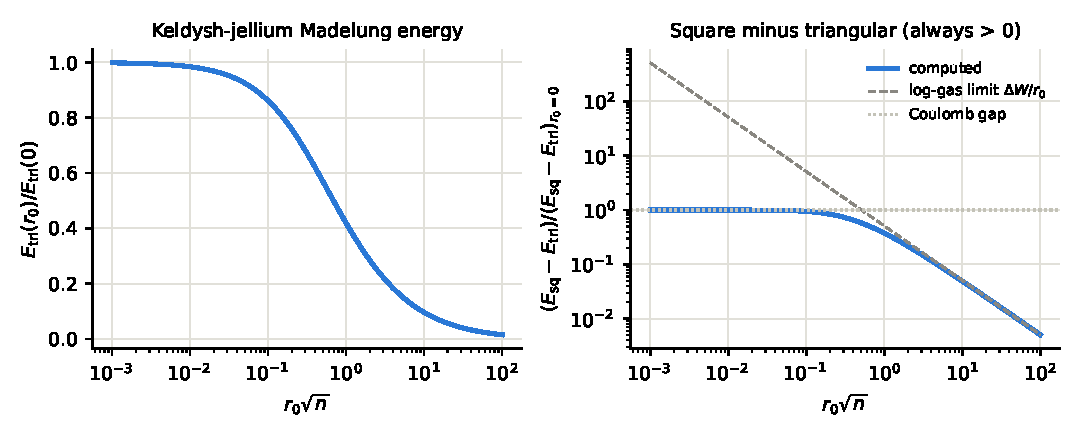
\includegraphics[width=\textwidth]{data/fig_keldysh_scan.pdf}
\caption{Keldysh-jellium Madelung energies at density one (\tier{X}), generated by
\texttt{scripts/keldysh/analyze.py} from \texttt{scan.json}. Left: $E_\mathrm{tri}(r_0)/E_\mathrm{tri}(0)$. This ratio
is dominated by the lattice-independent $+\pi\rho r_0$ background term, which comes from the neutralisation convention,
not from lattice structure. Right: the square--triangular gap, normalised by its Coulomb value, together with the
log-gas asymptote $\Delta W/r_0$. The panel title ``always $>0$'' is baked into the figure. It means positive at the
\KTNScan{} sampled points only.}\label{fig:scan}
\end{figure}

\paragraph{Materials.} We take $r_0=2\pi\chi_{2D}$ with the DFT+RPA polarizabilities of Table~I of~\cite{bhr}: 6.60,
8.23, 6.03 and 7.18~\AA{} for MoS$_2$, MoSe$_2$, WS$_2$ and WSe$_2$. We also use the MoS$_2$ GW value of 5.0~\AA{}
\tier{L, KT-L-0002}. Energies are converted with $e^2/(4\pi\varepsilon_0)=14.3996454687$~eV\,\AA{}, the scipy.constants
value. Table~\ref{tab:mat} and Figure~\ref{fig:mat} give the results \tier{X, KT-X-0007}. At $n=10^{11}$~cm$^{-2}$,
MoS$_2$ gives $E_\mathrm{tri}=\KTMoSElevenTri$~meV and a gap of \KTMoSElevenGap~meV. Relative to Coulomb at the same
density, the magnitude of $E_\mathrm{tri}$ is lower mostly because of the lattice-independent $+\pi\rho r_0$ background
term, which comes from the neutralisation convention rather than from lattice structure (as in
Figs.~\ref{fig:scan} and~\ref{fig:mat}). The structure-sensitive gap $E_\mathrm{sq}-E_\mathrm{tri}$ is also lower.

\begin{table}[h]\centering\small
\caption{Vacuum Keldysh-jellium Madelung energies per electron at $n=10^{12}$~cm$^{-2}$ (\tier{X}; $r_0$ \tier{L}).}\label{tab:mat}
\begin{tabular}{lrrrrr}\toprule
material & $r_0$ (\AA) & $r_0\sqrt n$ & $E_\mathrm{tri}$ (meV) & $E_\mathrm{tri}^{\rm Coulomb}$ (meV) & $E_\mathrm{sq}-E_\mathrm{tri}$ (meV)\\\midrule
\tabinput{gen/table_materials.tex}\bottomrule\end{tabular}
\end{table}

\begin{figure}[h]\centering
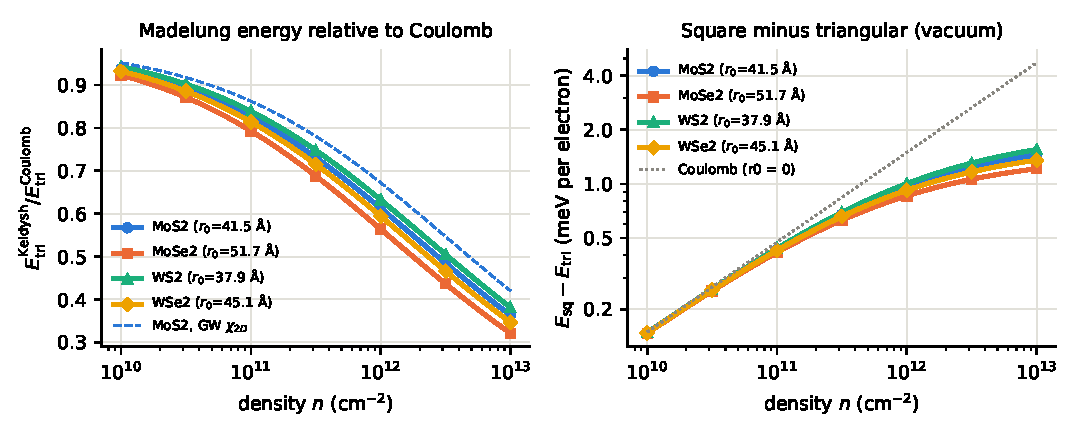
\includegraphics[width=\textwidth]{data/fig_keldysh_materials.pdf}
\caption{Material curves in vacuum (\tier{X}, with $r_0$ from~\cite{bhr} \tier{L}). Left: $E_\mathrm{tri}$ relative to
Coulomb. Like Fig.~\ref{fig:scan} (left), it is dominated by the $+\pi\rho r_0$ background term. Right: the
square--triangular gap in meV per electron. The density range $10^{10}$--$10^{13}$~cm$^{-2}$ is illustrative only. No
substrate or hBN is modelled.}\label{fig:mat}
\end{figure}

\section{HuggingFace dataset illustration}\label{sec:hf}
\emph{Search.} 23 Hub searches, 22 distinct terms (11 listed in \texttt{hf-data/keldysh\_tmd/search.json} and 12 in
\texttt{search2.txt}, with ``c2db'' repeated), found no dataset carrying a 2D polarizability $\alpha_{2D}$ or $\chi_{2D}$. \emph{Dataset used.} \texttt{colabfit/JARVIS\_C2DB} at revision
\texttt{432aeba9e505b59d0b3605c6346ac3816c754c02}, licence CC-BY-4.0. Its README cites Haastrup et
al.~\cite{c2db} and ColabFit~\cite{colabfit} \tier{L, KT-L-0005}. Files read: \texttt{README.md}, \texttt{ds.parquet},
\texttt{co/co\_0.parquet} (1.98~MB). It has 3520 configurations, with DFT-PBE energy and band gap only.

\emph{What it shows.} We use it only to \emph{identify} the 2H monolayers: three sites, a hexagonal cell, and both
chalcogens at the same in-plane point. We also cross-check lattice constants against the experimental values in Table~II
of~\cite{bhr} (Table~\ref{tab:hf}) \tier{X, KT-X-0008}. The PBE constants exceed experiment by 0.6--0.9\%. The rows
that pass the 2H test are the gapped ones, which is consistent with the 2H phase, but the gap was not the selection
criterion.

\emph{Caveats.} The dataset supplies no input to the energies; $r_0$ comes from~\cite{bhr}. C2DB itself publishes
$\alpha_{2D}$, but it is not on the Hub and was not downloaded.

\begin{table}[h]\centering\small
\caption{2H rows identified in \texttt{colabfit/JARVIS\_C2DB} (\tier{X}).}\label{tab:hf}
\begin{tabular}{llrrr}\toprule
material & row & $a$ PBE (\AA) & $a$ expt.~\cite{bhr} (\AA) & PBE gap (eV)\\\midrule
\tabinput{gen/table_hf.tex}\bottomrule\end{tabular}
\end{table}

\section{Claim ledger}\label{sec:ledger}
\texttt{ledger/build\_ledger.py} files 30 claims: 9 at Tier~A, 5 at L, 6 at C and 10 at X. Each claim has a
content-addressed evidence blob in \texttt{ledger/evidence/}:
\begin{itemize}
\item Tier A: verbatim axiom lines and source hashes;
\item Tier L: verbatim excerpts, in \texttt{ledger/sources/excerpts.json};
\item Tier C: argument text;
\item Tier X: result files with \texttt{claim\_licence: false}.
\end{itemize}
The Elenchus gate (\texttt{tools/ledger.py ledger.json -{}-evidence-dir evidence}) exits with code~1. It reports
\textbf{0 blocking findings} and \textbf{9 flags}, all \texttt{LEDGER\_UNAUDITED\_TIER\_A}: no person has certified that
the Tier~A statements mean what their glosses say. The flags remain open.

\section{Limitations}\label{sec:lim}
\begin{itemize}
\item \textbf{Upstream dependence.} Every triangular-lattice statement depends on openai/math's
\lean{universal\_energy\_minimum} (AI-generated, not peer reviewed) and on the fidelity of its definitions.
\item \textbf{Definition fidelity.} \lean{keldysh} is \emph{defined} by the mixture. The identification with
$\mathbf H_0-Y_0$ (Theorem~\ref{thm:ident}) is \tier{C}. Its main route rests on DLMF 11.5.2 \tier{L} and on the
subordination formula, which we use without a citation and check only numerically.
\item \textbf{Possibly empty corollaries.} The raw corollary is expected to be $\top\le\top$. The regularised one lacks a
finiteness proof.
\item \textbf{Two lattices only.} The jellium numerics compare triangular with square, in vacuum, as static classical
lattices.
\item \textbf{Producer $\ne$ verifier is still open.} The paper-stage reruns (Section~\ref{sec:repro}) were done by
another AI agent instance in the same workflow. A Stage-4 audit by a further AI agent instance recompiled
\texttt{Yukawa.lean} and \texttt{KeldyshCM.lean} into a private olean directory (rc~0, axioms within the allowlist, its
own planted \lean{sorry} and planted axiom caught), reran the scan (bit-identical) and the crate tests (28 passed, 0
failed, 1 ignored), and checked the citations (\texttt{AUDIT.md}). None of this is independent human verification, and
the human proofs are unrefereed.
\item \textbf{Novelty.} Complete monotonicity of $V$ follows from textbook integrals (Step~7(a)). Our alphaXiv search
did not find it stated, but that is weak evidence.
\item \textbf{Dependency drift.} The imported \texttt{Yukawa.lean} belongs to another lane (sha256 below). If it changes,
KeldyshCM must be rebuilt.
\end{itemize}

\section{Reproducibility}\label{sec:repro}
AutoevolveAI files are uncommitted on top of base \texttt{db794dd98d12c2a79702eab5651ae7c36a35ea27} (branch
\texttt{worktree-openai-math-discovery}). Source hashes (sha256):
\begin{itemize}\small
\item \texttt{KeldyshCM.lean}:\newline\texttt{\KTShaKeldysh}
\item \texttt{KeldyshCMControls.lean}:\newline\texttt{\KTShaControls}
\item \texttt{Yukawa.lean}:\newline\texttt{\KTShaYukawa}
\end{itemize}
Rust: rusty-SUNDIALS commit \texttt{2e41505cc9df8c46d2b2d667c89ea53e977218ca}, not pushed.
\begin{lstlisting}[basicstyle=\ttfamily\scriptsize]
taskset -c 4-7 python3 scripts/certified_numerics/lean_pinned.py compile formal_cert/Autoresearch/KeldyshCM.lean \
  --olean Autoresearch.KeldyshCM --json-out results/autoresearch/2026-10-25/H3/contribution/compile_keldysh.json
taskset -c 4-7 python3 scripts/certified_numerics/lean_pinned.py compile formal_cert/Autoresearch/KeldyshCMControls.lean \
  --json-out results/autoresearch/2026-10-25/H3/contribution/compile_controls.json
CARGO_TARGET_DIR=... cargo test --release -j 2 --offline --manifest-path <rusty-wt>/Cargo.toml -p qf-yukawa-crystal \
  -- --test-threads=2
keldysh_jellium scan results/keldysh/scan.json
python -I scripts/keldysh/analyze.py final results/keldysh <hf-data>/keldysh_tmd/tmd_rows.json
python -I papers/ar_keldysh_tmd/gen_inputs.py ; python -I papers/ar_keldysh_tmd/ledger/build_ledger.py
python3 <elenchus>/tools/ledger.py papers/ar_keldysh_tmd/ledger/ledger.json \
  --evidence-dir papers/ar_keldysh_tmd/ledger/evidence
\end{lstlisting}
\emph{Paper-stage reruns} (\tier{X, KT-X-0009}). These were run by a separate agent instance, not by a person:
\begin{itemize}
\item crate tests: \KTTestsPassed{} passed, \KTTestsFailed{} failed, \KTTestsIgnored{} ignored (the ignored test
predates this work);
\item \texttt{keldysh\_jellium scan}: output \KTScanSame{} to Stage~2's \texttt{scan.json};
\item Lean recompile of \texttt{KeldyshCM.lean}: \KTRecompileStatus.
\end{itemize}

\begin{thebibliography}{99}\small
\bibitem{bhr} T.~C. Berkelbach, M.~S. Hybertsen, D.~R. Reichman, \emph{Theory of neutral and charged excitons in
monolayer transition metal dichalcogenides}, arXiv:1305.4972v1 (2013).
\bibitem{keldysh} L.~V. Keldysh, JETP Lett.\ \textbf{29}, 658 (1979). Cited as reference [26] of~\cite{bhr}; not read
directly.
\bibitem{cudazzo} P.~Cudazzo, I.~V. Tokatly, A.~Rubio, Phys.\ Rev.\ B \textbf{84}, 085406 (2011). Cited as reference
[27] of~\cite{bhr}; not read directly.
\bibitem{ss} E.~Sandier, S.~Serfaty, \emph{From the Ginzburg--Landau model to vortex lattice problems},
arXiv:1011.4617v2 (2012).
\bibitem{dlmf} NIST Digital Library of Mathematical Functions, \S11.2 (Eq.~11.2.5) and \S11.5 (Eq.~11.5.2),
\url{https://dlmf.nist.gov/11}, read 2026-10-25.
\bibitem{oai} OpenAI, \emph{Universal optimality of the triangular lattice}, OpenAI Math release, github.com/openai/math,
commit \texttt{fd4aeeb2ee4fc729c18d98444fed42fd0529eeeb} (2026). AI-generated; not peer reviewed. The commit id is
inherited from the earlier published ledger; the pinned local copy has no \texttt{.git}, so it was not re-verified here.
\bibitem{bm77} L.~Bonsall, A.~A. Maradudin, Phys.\ Rev.\ B \textbf{15}, 1959 (1977), doi:10.1103/PhysRevB.15.1959, as
filed in the ledger of~\cite{uot} (UO-L-0007).
\bibitem{alves} Alves et al., Phys.\ Rev.\ B \textbf{103}, 245125 (2021), doi:10.1103/PhysRevB.103.245125, as filed in
the ledger of~\cite{uot} (UO-L-0007).
\bibitem{c2db} S.~Haastrup et al.\ (C2DB), doi:10.1088/2053-1583/aacfc1. Cited from the dataset README; title and journal
not verified by us.
\bibitem{colabfit} Haastrup et al., \emph{JARVIS C2DB}, ColabFit (2023), doi:10.60732/37c26dae; HuggingFace
\texttt{colabfit/JARVIS\_C2DB}, revision \texttt{432aeba9e505b59d0b3605c6346ac3816c754c02}.
\bibitem{uot} X.~Callens, \emph{Planar universal optimality, tiered}, preprint v2, doi:10.5281/zenodo.23293429 (2026).
\bibitem{txt} X.~Callens, \emph{The triangular lattice and universal optimality} (textbook),
doi:10.5281/zenodo.23295142 (2026).
\end{thebibliography}
\noindent This preprint applies the approach of~\cite{uot,txt}, kernel-checked consequences of upstream for explicit interactions, to
the Rytova--Keldysh interaction.
\end{document}
